\documentclass[../memoria.tex]{subfiles}

\begin{document}
\label{trabajo relacionado}

\indent En este capítulo se presenta una discusión de distintos métodos de Re-ID de personas, los que agruparemos según dos criterios: el tipo de características empleadas para construir el descriptor, y la técnica utilizada para asociar descriptores. 

%EXPLICAR QUE ES UN SISTEMA DE REID, ANTES DE DECIR COMO EVALUARLO
%HABLAR DE GALERIAS ABIERTAS (TRABAJO RELACIONADO) Y CERRADAS (MI TRABAJO)

\indent La efectividad de un sistema de Re-ID se evalúa mediante una curva CMC (\emph{Cumulative Matching Characteristic}), que mide la probabilidad de que el sistema entregue correctamente el descriptor que corresponde al descriptor consultado, donde la respuesta está compuesta por $k$ candidatos, y es considerada correcta si el descriptor que hace match con la consulta está entre dichos candidatos \cite{decann2012can}. Luego, CMC indica la proporción de respuestas correctas obtenidas para distintos valores de $k$:$${\rm\ Precisi\acute{o}n} = \frac{{\rm \#\ respuestas\ correctas}}{{\rm\ \#\ consultas\ realizadas}}\times 100$$

\section{Características empleadas}
\begin{figure}
  \centering
  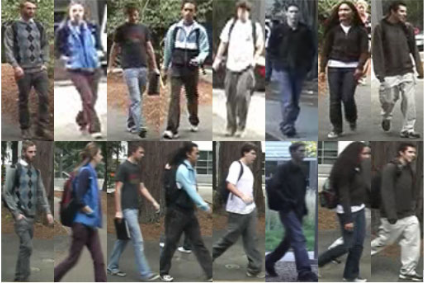
\includegraphics[width=0.5\textwidth]{viper.png}
  \caption{Ejemplos Data Set VIPeR: cada columna muestra una de las 632 personas.}
  \label{fig:viper}
\end{figure}
\indent Color, textura y forma son las características de apariencia comúnmente usadas por los métodos del estado del arte para Re-ID de personas, siendo algunas veces combinadas para obtener un descriptor más representativo \cite{mazzon2012person}. 

\subsection{Color}
\indent El color como característica de apariencia se ha empleado en forma de histogramas \cite{gheissari2006person, gray2008viewpoint, javed2008modeling, oliveira2009people, farenzena2010person, prosser2010person, zheng2011person}, dada la facilidad para calcularlos. Se pueden utilizar diferentes canales de colores y sus combinaciones. Por ejemplo, del espacio de colores HSV, se ha empleado sólo el tono \cite{oliveira2009people},  tono y saturación \cite{gheissari2006person}, o los tres canales del espacio \cite{farenzena2010person}. Por otro lado, histogramas del espacio de colores RGB fueron utilizados en \cite{prosserxiang2008multi, javed2008modeling, berdugo2010object}. Otros\cite{gray2008viewpoint, prosser2010person, zheng2011person} han adoptado una concatenación de histogramas de los canales de los espacios RGB, YCbCr y HSV (sólo tono y saturación). En \cite{gray2008viewpoint}, presentaron un dataset (VIPeR) conformado por 632 personas, cada una de ellas fotografiadas (48x128 píxeles) en ambientes exteriores, siempre desde dos ángulos distintos y en diferentes posiciones (ver figura \ref{fig:viper}). Las pruebas determinan que los canales más discriminantes (en orden descendente) para Re-ID personas, son: tono, saturación, azul, rojo y verde \cite{mazzon2012person}. Por último, pruebas de Re-ID con el dataset VIPeR utilizando descriptores compuestos únicamente por histogramas de colores y comparándolos con distancia euclidiana, para rangos $k=1$ y $k=20$ en la curva CMC, se obtiene un 6\% y 38\% de precisión de reconocimiento, respectivamente \cite{hirzer2012relaxed}.


\begin{figure}
  \centering
  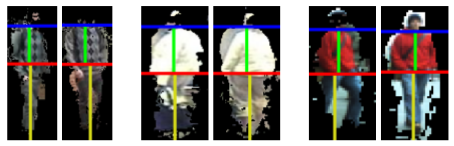
\includegraphics[width=0.6\textwidth]{sdalf.png}
  \caption{Algoritmo SDALF: Segmentación de la imagen usando ejes horizontales (partes asimétricas) y verticales (partes simétricas).}
  \label{fig:sdalf}
\end{figure}


\subsection{Forma}
\indent Se han propuesto algoritmos que hacen uso de la simetría de la figura humana \cite{farenzena2010person}: \emph{Symmetry-Driven Accumulation of Local Features}, SDALF. El método segmenta la silueta de la persona en tres partes: cabeza, torso y piernas (ver figura \ref{fig:sdalf}), comparando cada parte con su homóloga correspondiente. Luego, se buscan ejes verticales de simetría para cada una de las partes mencionadas, con el objetivo de ponderar las features (histogramas del espacio HSV de subregiones de píxeles) en relación a la distancia de éstas con el eje, destacando aquellas features que estén cercanas al eje, dado que tienen menor probabilidad de pertenecer al segundo plano de la imagen. Una evaluación de SDALF con el dataset VIPeR, obtiene para $k=1$ y $k=20$ en la curva CMC, un 20\% y 65\% de precisión de reconocimiento, respectivamente \cite{farenzena2010person}. %Un enfoque similar fue presentado en \cite{park2006vise}, donde se extraen tres histogramas para modelar cabeza, torso y piernas por separado.


\subsection{Textura}
%SVM y SIFT \cite{teixeira2009video}, Re-ID con SIFT \cite{hu2008people, martinel2012re}
\begin{table}
  \begin{center}
    \begin{tabular}{cccc}
      \hline
      Escena    & personas  & ocurrencias & exactitud \\
      \hline
      Salón     & 12        & 80          & 89.3\% \\
      Corredor  & 58        & 38          & 70.4\% \\
      Camino    & 10        & 20          & 95.0\% \\
      Cancha    & 6         & 106         & 85.9\% \\
      \hline
    \end{tabular}  
  \end{center}
  \caption{Resultados obtenidos en  \cite{hu2008people}}
\label{resultados SIFT hu2008}
\end{table}
\indent Algunos enfoques buscan Re-ID personas que abandonan y luego reingresan al FOV de una misma cámara, buscando enfrentar de forma robusta, cambios de iluminación, postura y escala \cite{hu2008people}. Para formar el descriptor de cada persona, se emplean histogramas de colores y características de textura seleccionadas por SIFT. Las pruebas se realizaron con videos\footnote{\url{http://groups.inf.ed.ac.uk/vision/CAVIAR/CAVIARDATA1/}} de cuatro escenarios distintos, donde aparece un grupo limitado de personas que abandonan e ingresan en reiteradas ocasiones, obteniendo una exactitud desde un 70.4\% hasta 95\% (ver cuadro \ref{resultados SIFT hu2008}). Un trabajo comparable a \cite{hu2008people} es presentado en \cite{hamdoun2008person}, donde se emplea el mismo dataset y método de extracción de características. La precisión de Re-ID obtenida en este trabajo depende de la cantidad mínima de keypoints coincidentes requeridos para establecer a sus respectivos descriptores como un match (ver cuadro \ref{resultados SIFT hamdoun2008person})  

\begin{table}
  \begin{center}
    \begin{tabular}{cc}
      \hline
      keypoint necesarios & Precisión \\
      \hline
      40 & 99\% \\
      30 & 95\% \\
      20 & 85\% \\
      10 & 10\% \\
      \hline
    \end{tabular}  
  \end{center}
  \caption{Resultados obtenidos en  \cite{hamdoun2008person}}
\label{resultados SIFT hamdoun2008person}
\end{table}


\section{Asociación de descriptores}

La segunda fase de un sistema de Re-ID define la forma de efectuar el match entre descriptores. Éstos se pueden asociar: (a) midiendo su similitud usando métricas de distancia directa, (b) utilizando algoritmos de aprendizaje supervisado y (c) aplicando métodos de optimización \cite{mazzon2012person}.
 
\subsection{Distancias directas}
Las métricas de distancia directas estiman diferencias entre descriptores. La métrica más usada es la distancia euclidiana, utilizada sobre descriptores basados en color \cite{farenzena2010person, bak2010person} y puntos de interés \cite{gheissari2006person}. 

%nota del profe: y? esto no dice nada
%Se han empleado otras funciones de distancia para medir similitud en sistemas de Re-ID, tales como: suma de distancias cuadráticas \cite{oliveira2009people}, suma de diferencias absolutas \cite{hamdoun2008person}, distancia  Bhattacharyya \cite{prosserxiang2008multi}, entre otras. 

%nota del profe: no aporta
%La selección de la métrica de distancia que mejor se ajuste a un conjunto de features específico se efectúa, generalmente, por ensayo y error \cite{mazzon2012person}. 

\indent Sin embargo, utilizar únicamente métricas de distancia directa no siempre permite establecer una correcta similitud entre descriptores, pues cuando la mayoría de las features de un descriptor coincide con los de otro correspondiente a una persona desigual, los descriptores respectivos estarán cercanos entre sí. Del mismo modo, para una misma persona que cambia de apariencia (cambio drástico en varios features a causa de diferente iluminación, postura de la persona, punto de vista, etc.), sus respectivos descriptores se encontrarán a mayor distancia. Como consecuencia, al emplear sólo una distancia tradicional, se ignora cualquier regularidad estadística, la que podría ser estimada con algoritmos de aprendizaje supervisados \cite{zheng2011person, prosser2010person}. Un sistema de Re-ID de personas que sólo emplea una métrica directa, no es robusto ante cambios de iluminación, razón por la que se requiere una calibración previa en la red de cámaras \cite{gilbert2006tracking, porikli2003multi, stein1999tracking, javed2008modeling}. %Como alternativa, un clasificador puede ser entrenado para aprender los cambios producidos entre cámaras.%Por otro lado, métodos que utilizan datos de entrenamiento (en este caso, la relación existente entre pares de imágenes), obtienen mejores resultados que otros métodos no basados en aprendizaje automático.

\subsection{Aprendizaje supervisado}

%MENCIONAR: \cite{gray2008viewpoint, prosser2010person, teixeira2009video, zheng2011person, hirzer2012person }

\indent Las técnicas de aprendizaje automático (Machine Learning, ML) se han empleado en sistemas de Re-ID para distintos objetivos. Por ejemplo, un clasificador binario puede distinguir entre descriptores positivos (match) y negativos (missmatch). Un sistema de Re-ID basado en SVM, puede etiquetar un par de descriptores como match incluso si éstos presentan más diferencias que otro par compuesto por descriptores de personas distintas \cite{prosser2010person}. El método anterior obtiene, para $k=1$ y $k=20$ en la curva CMC, un 14\% y 68\% de precisión en reconocimiento, respectivamente.

%nota del profe: no aporta
%%\begin{figure}[h]
%%  \centering
%%  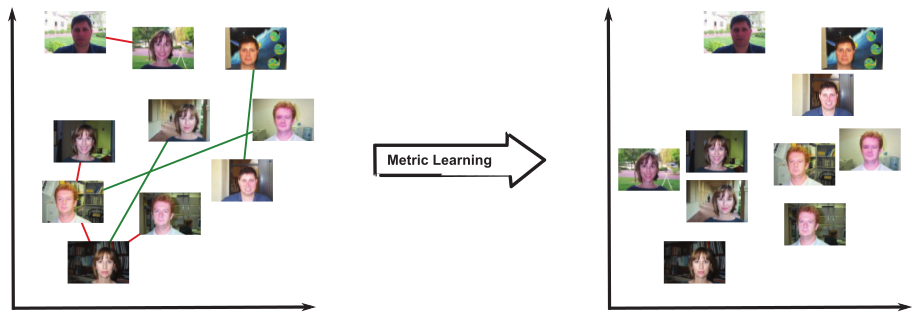
\includegraphics[width=\textwidth]{distancias.png}
%%  \caption{Objetivo de un algoritmo de Aprendizaje de Métricas de Distancia \cite{bellet2013survey}.}
%%  \label{fig:dml}
%%\end{figure}

%ELF
\indent Un algoritmo clásico (AdaBoost) \cite{gray2008viewpoint},  que selecciona las características que determinan una mayor diferencia entre pares de imágenes, con base en pares etiquetados de imágenes, obteniendo un 12\% y 60\% en la curva CMC para rangos de $k=1$ y $k=20$, respectivamente. 

%DML
\indent También, se ha empleado ML para aprender funciones de similitud o distancia (Distance Metric Learning o DML). El objetivo es encontrar un espacio geométrico donde descriptores de una misma persona queden a poca distancia, al mismo tiempo que descriptores de personas distintas estén a una distancia mayor \cite{bellet2013survey}. Una variante de este método establece distancias de forma relativa a un tercer descriptor, por ejemplo, indicando que $A$ está más cerca de $B$ que de $C$ \cite{zheng2013reidentification}. Esto obtiene, para $k=1$ y $k=20$ en la curva CMC, un 15.7\% y 70.1\% de precisión de reconocimiento, respectivamente.  

%% LMMN
\indent Otros métodos \cite{weinberger2008fast} utilizan el espacio geométrico obtenido con un algoritmo DML, en un clasificador kNN. Los resultados muestran un 18\% y 75\% de precisión de reconocimiento para $k=1$ y $k=20$ en la curva CMC, respectivamente \cite{hirzer2012relaxed}. Mejoras al enfoque anterior consideran la capacidad de rechazar %explicar que es rechazar. Idea de contextualización: cómo funcionan los sistemas de reid: con una galeria, abierta (novelti detection) o cerrada (no se agregan nuevos descriptores). Explicar cada una. definir el tipo de sistema a implementar
del clasificador (detectar una pareja negativa) \cite{dikmen2011pedestrian}. Para esto, es necesario establecer una distancia umbral, tal que, el elemento consultado es aceptado sólo si existe un vecino cuya distancia es inferior a dicho umbral. En otro caso, el elemento consultado es rechazado. Los resultados obtenidos para $k=1$ y $k=20$, alcanzan aproximadamente un 20\% y 80\% de precisión de reconocimiento, respectivamente \footnote{\label{lmnn-r}Resultados obtenidos por la mejor ejecución, a diferencia de otros trabajos donde los autores muestran un promedio de los experimentos realizados}. %También se ha utilizado \cite{hirzer2012relaxed} un sistema basado en aprendizaje de métrica y aplicarla en un clasificador kNN. A diferencia de \cite{weinberger2008fast}, la métrica cumple los requerimientos de distancia de forma más aproximada, obteniendo los mejores resultados que trabajos anteriores: 27\% y 83\% de precisión de reconocimiento en la curva CMC, para rangos $k=1$ y $k=20$. Para evaluar que tan sobre-ajustado está el modelo, se redujo la cantidad de datos de entrenamiento \cite{zheng2013reidentification, hirzer2012relaxed}. Aunque el rendimiento se vio afectado, aún era superior al obtenido por métodos que sólo emplean distancias tradicionales. %Esto se puede deber a que DML logra obtener el patrón existente en los datos, que permite establecer la distancia deseada entre nuevos elementos.

%DESVENTAJA
\indent A diferencia de métricas directas, los métodos que utilizan DML son menos sensibles a las features seleccionadas. Sin embargo, en escenarios reales no siempre se cuenta con un conjunto de datos previamente etiquetados para entrenar el sistema.


\subsection{Optimización Convexa}
En este tipo de métodos, la búsqueda de la métrica se hace por medio de un modelo de optimización convexa, donde la función objetivo consiste en minimizar de la distancia entre pares descriptores que hagan match, con la restricción de mantener una distancia mínima entre descriptores de pares mismatch \cite{javed2008modeling, kuo2010inter, porikli2003multi}. La principal desventaja de este enfoque es el costo computacional, debido a la cantidad de restricciones y al tamaño de cada descriptor. %los enfoques basados en la optimización, es que operan sobre datos por lotes y no se pueden ejecutar en tiempo real. Sin embargo, en las restricciones se pueden incluir features espacio-temporales de personas que transitan por la red de cámaras. Se alcanzan resultados usualmente sobre 90\% \cite{javed2008modeling} de precisión de reconocimiento para $k=1$ en la curva CMC en escenas con visibilidad completa del cuerpo y una transición lineal en regiones fuera del FOV.


\begin{table}
  \begin{center}
    \begin{tabular}{|l|ccc|ccc|}
      \hline
      \multirow{2}{6em}{Referencia} & \multicolumn{3}{c|}{Características} & \multicolumn{3}{c|}{Asociación} \\     
      & Color & Textura & Forma & Distancia & Aprendizaje & Optimización \\
      \hline
      \cite{bak2010person, farenzena2010person, gheissari2006person, oliveira2009people} & \checkmark & \checkmark & &\checkmark & & \\
      \cite{bauml2010multi} & & \checkmark & & & \checkmark & \\
      \cite{berdugo2010object,wang2007shape} & \checkmark & \checkmark & \checkmark & \checkmark & & \\
      \cite{gray2008viewpoint, prosser2010person, zheng2011person} & \checkmark & \checkmark & & & \checkmark & \\
      \cite{hamdoun2008person} & & \checkmark & & \checkmark & & \\
      \cite{hirzer2012person} & \checkmark & & & & \checkmark & \\
      \cite{javed2008modeling, porikli2003multi} & \checkmark & & & & & \checkmark \\
      \cite{kuo2010inter} & \checkmark & \checkmark & \checkmark & & & \checkmark \\
      \cite{prosserxiang2008multi} & \checkmark & & & \checkmark & & \\
      \cite{teixeira2009video} & & \checkmark & & & \checkmark & \\
      \hline
    \end{tabular}  
  \end{center}
  \caption{Clasificación de trabajos en tipos de métodos de Re-ID \cite{mazzon2012person}}
\label{estado-arte-re-id}
\end{table}

\end{document}
